\section{Assoziationsklasse (Attributierte Assoziation)}

\begin{tcolorbox}[title=Assoziationsklasse (Attributierte Assoziation)]
Eine \textbf{Assoziationsklasse} erlaubt das Hinzufügen von Operationen und Attributen zu einer Assoziation (\cite[43]{Buh09}).\\
Assoziationsklassen werden in der \textbf{Analyse} in Modellen verwendet und in dem \textbf{Entwurf} in eigenständige Klassen transformiert.\\


\blockquote[{\cite[277]{Oes05}}]{
    Eine attributierte Assoziation ist immer dann nahe liegend, wenn Attribute oder Operationen gefunden werden, die weder der einen noch der anderen Klasse zugeordnet werden können, weil sie nämlich Eigenschaften der Beziehung selbst sind.
}.\\

Bei einer attributierten Assoziation dürfen zwei beteiligte Objekte maximal nur eine Beziehung zueinander haben (vgl.~\cite[277]{Oes05})\footnote{
    \textit{Ostereich} führt dies ebenda auf Seite 278 weiter aus, in dem er beschreibt, wie eine attributierte Assoziation für ein \textit{Beschäftigtenverhältnis} zwischen \textit{Mitarbeiter} und \textit{Unternehmen} modelliert wird. Dabei wird davon ausgegangen, dass ein \textit{Mitarbeiter} nur über \textit{ein} Arbeitsverhältnis mit einem \textit{Unternehmen} in Beziehung stehen kann. Bestehen mehrere Arbeitsverhältnisse (\textit{Mitarbeiter} hat zu unterschiedlichen Zeitpunkten für das \textit{Unternehmen} gearbeitet), kann die attributierte Assoziation nicht verwendet werden.\\

\noindent
Wird eine attributierte Assoziation in eine gewöhnliche Assoziation transformiert, muss darauf geachtet werden, die Multiplizitäten richtig zu setzen (s. Abbildung~\ref{fig:assoziationsklasse}).
\end{tcolorbox}

\begin{figure}
    \centering
    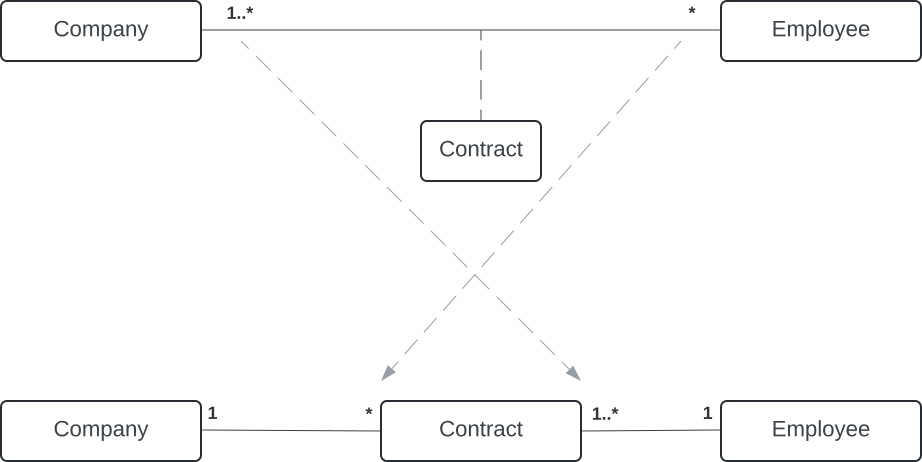
\includegraphics[scale=0.4]{part three/Klassendiagramme - Erweiterte Konzepte und Paketdiagramme/img/assoziationsklasse}
    \caption{Darstellung einer Assoziation mit Hilfe einer Assoziationsklasse (oben) sowie Transformation in gewöhnliche Assoziationen (unten). (Quelle: in Anlehnung an \cite[279, Abb. 4.4-11]{Oes05})}
    \label{fig:assoziationsklasse-cc}
\end{figure}
